
To this date, sustainable energy sources have become an area in focus worldwide in an attempt to reduce the environmental impact due to emissions of CO2 and other greenhouse gasses. The development of competitive systems to exploit renewable energy sources is the best alternative to reduce the use of fossil fuels for the production of electricity. Over the last years there have been a considerable increase in electricity production from renewable energy sources being the fastest growing sector wind and solar energy. In 2017, solar photovoltaic was the renewable energy source which experienced the highest increased in newly installed capacity amounting a total installed capacity of approximately 402 GW. %[http://www.ren21.net/wp-content/uploads/2018/06/17-8652_GSR2018_FullReport_web_-1.pdf] 

Photovoltaic (PV) is referred to the production of electricity in the form of direct current (DC) directly from sunlight shining on solar cells. Solar cells are semiconductor devices which typically can produce around 0.5 V DC so they are series connected to form a PV module/panel which can also be connected to other PV panels resulting in a PV array. This way, according to the system´s requirements, the PV panels can be interconnected in series or parallel in order to get at the output a higher voltage or current, respectively. Connecting PV panels either in series or parallel will result in an increase of the system´s overall electricity production. %[http://www.sabz-energy.com/solar%20electricity%20handbook%202017.pdf] 

Nevertheless, it is essential to keep into consideration the mismatches that may appear between the power generated by the different PV panels, which will result in losses in the PV system and thus in a lower efficiency. Mismatches occur when the PV modules operate in a different operating point than its maximum power point (MPP) due to partial shading, manufacturing tolerances, defects in the PV modules due to weather conditions and aging, among others. Mismatch losses in a PV system can be reduced by forcing every PV module to work at its MPP by using a technique known as Maximum Power Point Tracking (MPPT). This can be reached by using electronic devices called Module Integrated Converters (MICs) which basically consist on DC-AC micro inverters or DC-DC converters with a MPPT unit to ensure that the output power of the MIC is the one corresponding to the MPP of the PV module.%[https://www.researchgate.net/publication/43248773_Study_on_MPP_mismatch_losses_in_photovoltaic_applications] 

This project focuses on the design and test of a MIC based on a non-inverting buck-boost DC/DC converter for integration with a PV module in order to operate at its MPP and thus harvest maximum energy from the sunlight. 

\section{PV generation}



\section{State of The Art}

Example of including a picture
\begin{figure}[htbp]
	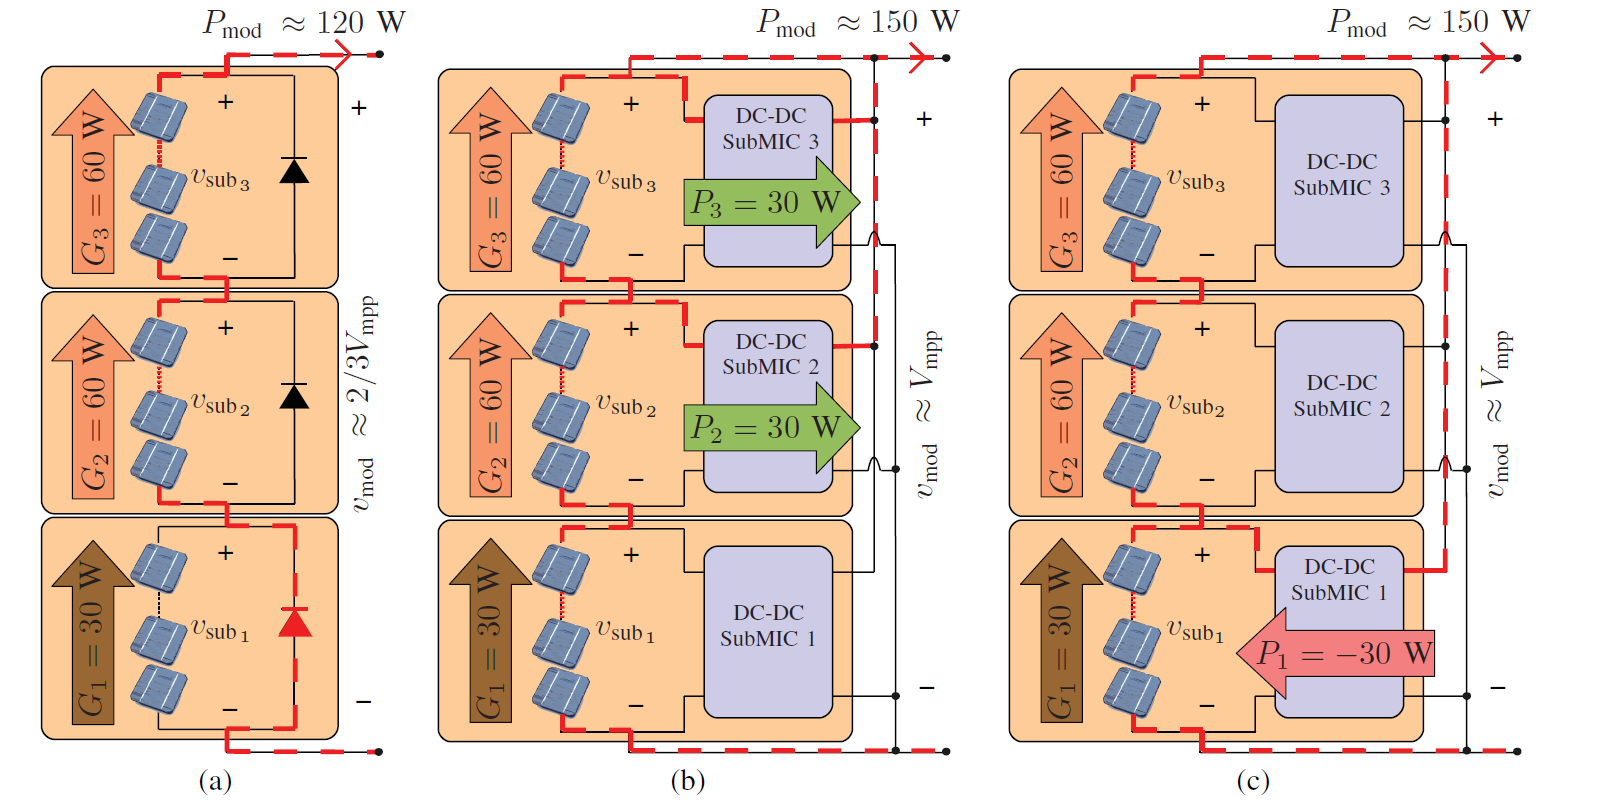
\includegraphics[width=\linewidth]{../Pictures/test.png}
	\caption{Functional flow block diagram}
	\label{fig:TimePlan}
\end{figure}

Example of creating a table \ref{table}.
\begin{table}[htbp]
	\begin{tabular}{|m{1.5cm}|m{8cm}|m{2.5cm}|m{2.5cm}|}
		\hline
		\rowcolor{lightgray} \textbf{ID} & \textbf{Technical Requirements}  & \textbf{Requirement Type}  &  \textbf{Verification Method}    \\ \hline
		AX-1 & The pod shall be center-mountable on the Royal Danish Air Force (RDAF) F-16 AM/BM fighter aircrafts in version M6.5     & M   & A      \\ \hline
		\rowcolor{Seashell2} AX-2 & The pod shall have a mass less than 700 pounds in total & M  & A        \\ \hline
		AX-3 & The pod shall have a geometric cross-section of $0.40m^2$  or less as seen from the front   &  M   & A                \\ \hline
		\rowcolor{Seashell2} AX-4 & The pod should have a geometric cross-section of $0.25m^2$ or less as seen from the front   &  D   &                \\ \hline
	\end{tabular}
	\caption{Flight requirements}
	\label{tab:TechRequirements}
\end{table}




